\chapter{Safety controllers}


\begin{description}
    \item[Control-affine non-linear dynamical system] \marginnote{Control-affine non-linear dynamical system}
        System whose dynamics follows:
        \[
            \dot{\x}(t) = f(\x(t)) + g(\x(t)) \u(t) \quad \x(0) = \x_0
        \]
        with $\x(t) \in \mathbb{R}^n$, $\u(t) \in U \subseteq \mathbb{R}^m$, $f(\x(t)) \in \mathbb{R}^n$, and $g(\x(t)) \in \mathbb{R}^{n \times m}$.

        $f(\x(t))$ can be seen as the drift of the system and $\u(t)$ as a coefficient that controls how much $g(\x(t))$ is injected into $f(\x(t))$.

        The overall system can be interpreted as composed of:
        \begin{itemize}
            \item A high-level controller that produces the direction $\u^\text{ref}(\x)$ towards the target position.
            \item A safety layer that modifies $\u^\text{ref}(\x)$ into $\u(t) = \kappa(\x)$ to account for obstacles.
        \end{itemize}

    \item[Safety control] \marginnote{Safety control}
        Given a (sufficiently regular) function $V^s: X \subseteq \mathbb{R}^n \rightarrow \mathbb{R}$, it is possible to define a safe state set as:
        \[
            X^s = \{ \x \in X \subseteq \mathbb{R}^n \mid V^s(\x) \geq 0 \}
        \]

        The goal is to design a feedback control law $\kappa^s: X \rightarrow \mathbb{R}^m$ for a control-affine non-linear dynamical system such that the set $X^s$ is forward invariant (i.e., any trajectory starting in $X^s$ remains in $X^s$).

        \begin{figure}[H]
            \centering
            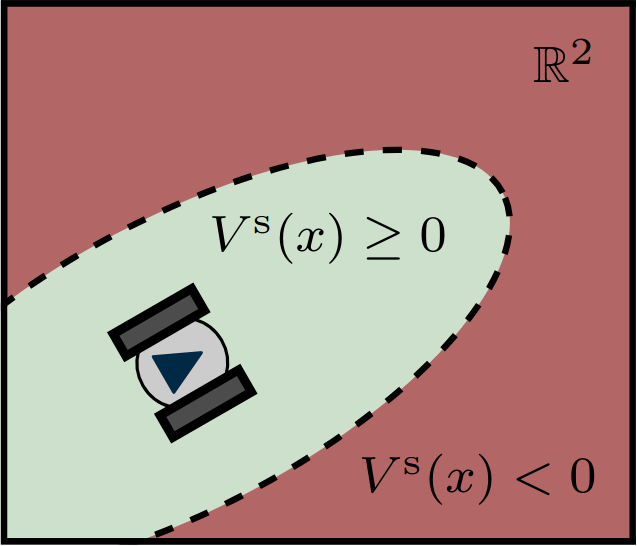
\includegraphics[width=0.25\linewidth]{./img/safety_control.png}
        \end{figure}

        \begin{remark}
            The time derivative of $V^s(\x(t))$ along the system trajectories is given by:
            \[
                \begin{split}
                    \frac{d}{dt} V^s(\x(t)) 
                    &= \nabla V^s(\x(t))^T \frac{d}{dt} \x(t) \\
                    &= \nabla V^s(\x(t))^T \Big( f(\x(t)) + g(\x(t)) \u(t) \Big) \\
                    &= \nabla V^s(\x(t))^T f(\x(t)) + \sum_{h=1}^{m} \Big( \nabla V^s(\x(t))^T g_h(\x(t)) \u_h(t) \Big)\\
                    &= L_f V^s(\x(t)) + L_g V^s(\x(t)) \u(t) \\
                \end{split}
            \]
            where $L_h V^s(\x(t)) = \nabla V^s(\x(t))^T h(\x(t))$ is the lie derivative.
        \end{remark}

    \item[Control barrier function (CBF)] \marginnote{Control barrier function (CBF)}
        A function $V^s$ is a control barrier function if there exists a continuous strictly increasing function $\gamma: \mathbb{R} \rightarrow \mathbb{R}$ with $\gamma(0) = 0$ such that the following inequality (control barrier certificate) holds:
        \[
            \sup_{\u \in U} \{ L_fV^s(\x) + L_gV^s(\x)\u + \gamma(V^s(\x)) \} \geq 0 \quad \forall \x \in X
        \]
        $\gamma$ can be interpreted as a degree of movement freedom since, as long as it holds that $V^s(\x(t)) > 0$, it is allowed that $\frac{d}{dt} V^s(\x(t)) < 0$ (i.e., the agent can move closer to the border between safe and unsafe region).

        \begin{remark}
            In principle, the negative part of $\gamma$ is not necessary (the agent should start in a safe area). However, as it is strictly increasing, it allows to move out the unsafe region if the agent ever ends up there.
        \end{remark}

        \begin{example}
            A simple choice for $\gamma$ is a linear function $\gamma(r) = \gamma r$ with $\gamma > 0$.
        \end{example}

    \item[Set of admissible safe controllers] \marginnote{Set of admissible safe controllers}
        The set of inputs that satisfy the control barrier certificate for a given state $\x$ is:
        \[
            U^s(\x) = \{ \u \in U \mid L_f V^s(\x) + L_g V^s(\x) \u + \gamma(V^s(\x)) \geq 0 \}
        \]
\end{description}


\section{Safety filter via control barrier certificate}

\begin{description}
    \item[Safety filter via control barrier certificate] \marginnote{Safety filter via control barrier certificate}
        Given a possibly unsafe reference input (from the high-level controller) $\u^\text{ref}(\x) \in \mathbb{R}^m$, the safety controller (i.e., rectifying controller) based on the control barrier certificate is designed to be minimally invasive (i.e., alter the reference as little as possible). 
        
        The policy $\u = \kappa^s(\x)$ can be defined as:
        \[
            \begin{gathered}
                \kappa^s(\x) = \arg\min_{\u \in U} \Vert \u - \u^\text{ref}(\x) \Vert^2 \\
                \text{subject to } -L_fV^s(\x) - L_gV^s(\x)\u - \gamma(V^s(\x)) \leq 0
            \end{gathered}
        \]

        \begin{remark}
            In the general case, this problem should be solved at each $t \geq 0$.
        \end{remark}


    \item[Single integrator model] \marginnote{Single integrator model}
        Control-affine non-linear dynamical system where $f(\x(t)) = 0$ and $g(\x(t)) = \matr{I}$. The dynamics is:
        \[
            \begin{split}
                \dot{\x} 
                &= 0 + \matr{I}\u \\ 
                &= \u
            \end{split}
        \]
        with $\x \in \mathbb{R}^d$ and $\u \in \mathbb{R}^d$.

        \begin{remark}
            In the case of single integrators, we have that:
           \begin{itemize}
            \item $L_f V^s(\x) = \nabla V^s(\x)^T 0 = 0$,
            \item $L_g V^s(\x) = \nabla V^s(\x)^T \matr{I} = \nabla V^s(\x)^T$.
           \end{itemize}
           Therefore:
           \[
                \begin{split}
                    \frac{d}{dt} V^s(\x(t)) 
                    &= L_f V^s(\x(t)) + L_g V^s(\x(t)) \u(t) \\
                    &= \nabla V^s(\x(t))^T \u(t)
                \end{split}
           \]
        \end{remark}
\end{description}


\subsection{Single-robot obstacle avoidance with single integrator models}

\begin{description}
    \item[Single-robot obstacle avoidance] \marginnote{Single-robot obstacle avoidance} 
        Task where the goal is to keep an agent to a safety distance $\Delta > 0$ from an obstacle.

        \begin{figure}[H]
            \centering
            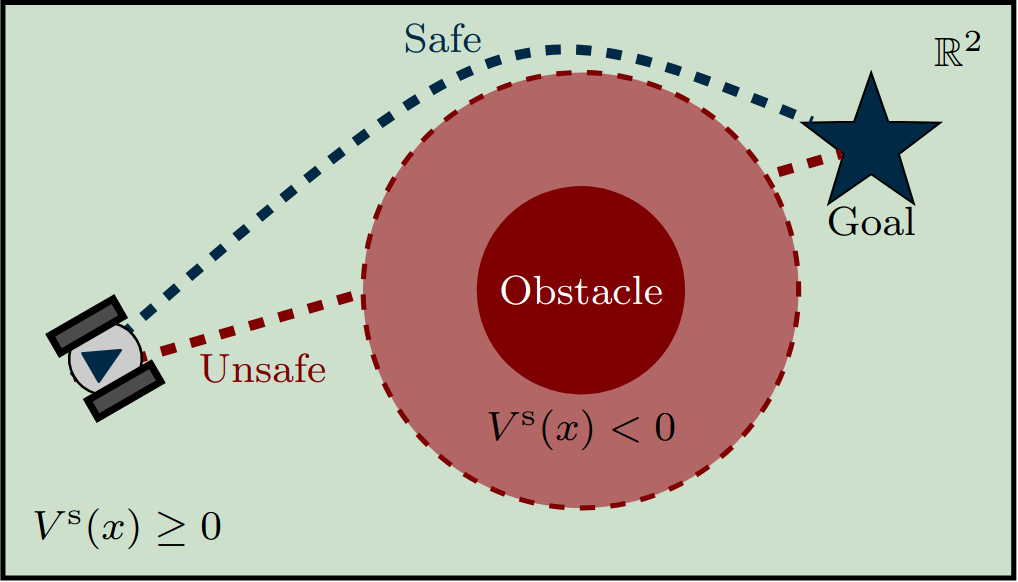
\includegraphics[width=0.35\linewidth]{./img/safety_control_single.png}
        \end{figure}

        A control barrier function to solve the task (i.e., rectify the trajectory of the high level controller) can be:
        \[
            V^s(\x) = \Vert \x - \x_\text{obs} \Vert^2 - \Delta^2
            \qquad
            \nabla V^s(\x) = 2(\x - \x_\text{obs})
        \]

        The CBF-based safety policy $\kappa^s(\x)$ can be obtained by solving:
        \[
            \begin{gathered}
                \arg\min_{\u \in U} \Vert \u - \u^\text{ref}(\x) \Vert^2 \\
                \text{subject to } -2(\x-\x_\text{obs})^T \u - \gamma(\Vert \x-\x_\text{obs} \Vert^2 - \Delta^2) \leq 0
            \end{gathered}
        \]

        As there are two constants in the constraint $a = -2(\x-\x_\text{obs})^T$ and $b = \gamma(\Vert \x-\x_\text{obs} \Vert^2 - \Delta^2)$, the problem can be reformulated as:
        % \[
        %     \arg\min_{\u \in U} \u^T\u - 2\u^T\u^\text{ref} \quad \text{subject to } a^T \u + b \leq 0
        % \]
        \[
            \arg\min_{\u \in U} \Vert \u - \u^\text{ref}(\x) \Vert^2 \quad \text{subject to } a^T \u + b \leq 0
        \]
        
        \begin{remark}
            If $U$ is a polytope (or unconstrained: $U = \mathbb{R}^d$), the problem becomes a quadratic program.
        \end{remark}
\end{description}


\subsection{Multi-robot collision avoidance with single integrator models}


\begin{description}
    \item[Multi-robot collision avoidance] \marginnote{Multi-robot collision avoidance}
        Task with $N$ single integrator agents that want to keep a safety distance $\Delta > 0$ among them.

        \begin{figure}[H]
            \centering
            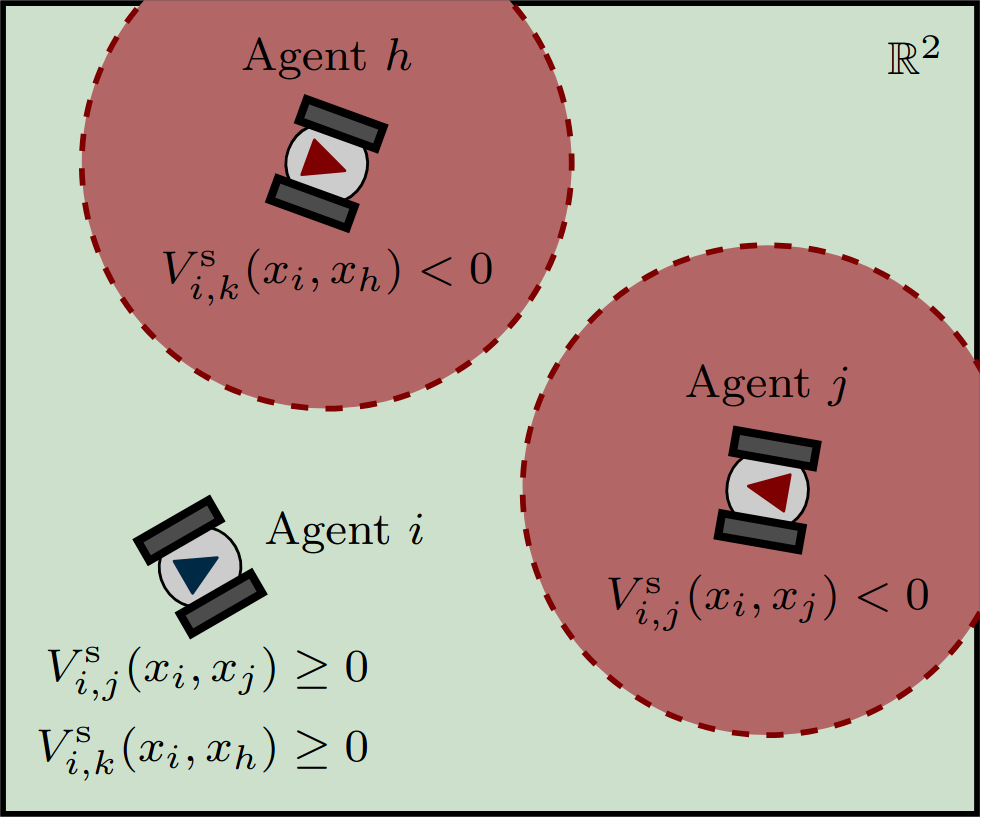
\includegraphics[width=0.35\linewidth]{./img/safety_control_multi.png}
        \end{figure}

        The local control barrier function to solve the task can be defined as:
        \[
            V^s_{i,j}(\x_i, \x_j) = \Vert \x_i - \x_j \Vert^2 - \Delta^2
            \qquad
            \begin{aligned}
                \nabla_{[\x_i]} V_{i,j}^s(\x_i, \x_j) &= 2(\x_i - \x_j) \\
                \nabla_{[\x_j]} V_{i,j}^s(\x_i, \x_j) &= 2(\x_j - \x_i)
            \end{aligned}
        \]
        The safe region $X_i$ for agent $i$ can be defined as:
        \[
            X_i = \{ \x \in \mathbb{R}^d \mid \forall j \in \mathcal{N}_i: V_{i,j}^s(\x) \geq 0 \}
        \]

        The set of admissible controllers is:
        \[
            \begin{aligned}
                \begin{aligned}
                    U^s(\x) = \Big\{ \u \in \mathbb{R}^{dN} \mid 
                    -\nabla_{[\x_i]} V_{ij}^s(\x_i, \x_j)^T \u_i 
                    - \nabla_{[\x_i]} V_{ji}^s(\x_j, \x_i)^T \u_j 
                    - &\gamma(V_{ij}^{s}(\x_i, \x_j)) \leq 0 \\
                    &\forall j \in \mathcal{N}_i, \forall i \in \{1, \dots, N\} \Big\}
                \end{aligned} \\
                = \Big\{ \u \in \mathbb{R}^{dN} \mid -2(\x_i-\x_j)^T \u_i - 2(\x_j-\x_i)^T \u_j - \gamma(V_{ij}^s(\x_i, \x_j)) \leq 0 \,\,\forall j \in \mathcal{N}_i, \forall i \in \{1, \dots, N\} \Big\}
            \end{aligned}
        \]

        % \[
        %     L_g V_{ij}^s(\x) = \nabla_{[\x_i]} V^s(\x_i, \x_j)^T \u_i + \nabla_{[\x_j]} V^s(\x_i, \x_j)^T \u_j
        % \]
\end{description}

\begin{description}
    \item[Centralized safety controller] \marginnote{Centralized safety controller}
        The CBF-based policy can be obtained by solving:
        \[
            \begin{gathered}
                \arg\min_{\u \in \mathbb{R}^N} \sum_{i=1}^{N} \Vert \u_i - \u_i^\text{ref} \Vert^2 \\
                \begin{aligned}
                    \text{subject to } 
                    &-2(\x_i-\x_j)^T \u_i - 2(\x_j-\x_i)^T \u_j - \gamma(V_{ij}^s(\x_i, \x_j)) \leq 0 \\
                    & \Vert \u_i \Vert \leq \u_i^\text{max} \\
                    & \forall j \in \mathcal{N}_i, \forall i \in \{ 1, \dots, N \}
                \end{aligned}
            \end{gathered}
        \]
        where $\u_i^\text{ref}$ is the reference input of the high level controller and $\u_i^\text{max}$ is the bound.

        \begin{remark}
            The policy should be computed continuously for each $\x_i(t)$.
        \end{remark}

    \item[Decentralized safety controller] \marginnote{Decentralized safety controller}
        The CBF-based policy can be obtained by solving a more constrained problem compared to the centralized formulation:
        \[
            \begin{gathered}
                \arg\min_{\u_i \mathbb{R}^d} \Vert \u_i - \u_i^\text{ref} \Vert^2 \\
                \begin{aligned}
                    \text{subject to } &- \nabla_{[\x_i]} V_{ij}^s(\x_i, \x_j)^T \u_i - \frac{1}{2} \gamma (V_{ij}^s(\x_i, \x_j)) \leq 0 \\
                    & \Vert \u_i \Vert \leq \u_i^\text{max} \\
                    & \forall j \in \mathcal{N}_i
                \end{aligned}
            \end{gathered}
        \]

        \begin{remark}
            If $\forall i \in \{1, \dots, N\}: \nabla_{[\x_i]} V_{ij}^s(\x_i, \x_j)^T \u_i \geq \frac{1}{2} \gamma (V_{ij}^s(\x_i, \x_j))$, then it holds that:
            \[
                \begin{split}
                    \nabla_{[\x_i]} V_{ij}^s(\x_i, \x_j)^T \u_i + \nabla_{[\x_i]} V_{ji}^s(\x_j, \x_i)^T \u_j 
                    &\geq -\frac{1}{2} \gamma\left( V_{ij}^s(\x_i, \x_j) \right) - \frac{1}{2} \gamma\left( V_{ji}^s(\x_j, \x_i) \right) \\
                    &\geq - \gamma\left( V_{ij}^s(\x_i, \x_j) \right)
                \end{split}
            \]
        \end{remark}
\end{description}


\subsection{Multi-robot collision avoidance with unicycle control}

\begin{description}
    \item[Unicycle model with non-holonomic constraints] 
        Model that captures the constraints given by wheels. Its dynamics is:
        \[
            \begin{split}
                \dot{\vec{p}}_x &= v \cos(\theta) \\
                \dot{\vec{p}}_y &= v \sin(\theta) \\
                \dot{\theta} &= \omega \\
            \end{split}
        \]
        where:
        \begin{itemize}
            \item $(\vec{p}_x, \vec{p}_y)$ is the position of the center of mass,
            \item $\dot{\theta}$ is the orientation,
            \item $v$ is the linear velocity,
            \item $\omega$ is the angular velocity.
        \end{itemize}

        \begin{figure}[H]
            \centering
            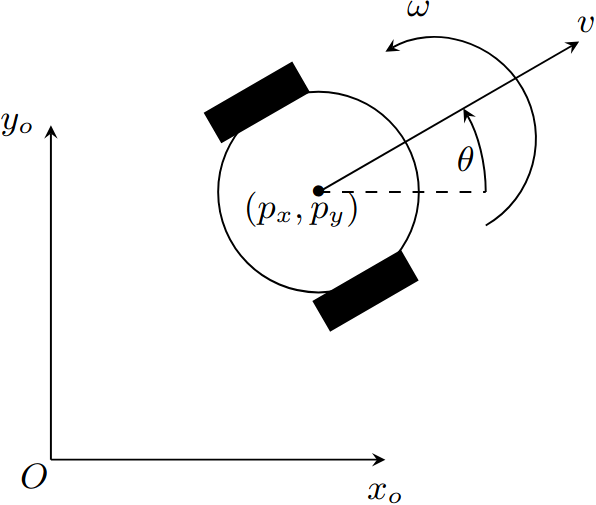
\includegraphics[width=0.25\linewidth]{./img/unicycle_model.png}
        \end{figure}

        \begin{remark}
            It is assumed that the robot does not drift sideways ($v_{\bot} = 0$).
        \end{remark}

    \item[Single integrator to unicycle control mapping] \marginnote{Single integrator to unicycle control mapping}
        Consider a point $\x^\text{int}$ longitudinal to $v$ that is not the barycenter:
        \[
            \x^\text{int} = \begin{bmatrix}
                \vec{p}_x \\ \vec{p}_y
            \end{bmatrix}
            +
            \rho \begin{bmatrix}
                \cos(\theta) \\ \sin(\theta)
            \end{bmatrix}
        \]
        where $\rho > 0$ is the distance to the barycenter.

        By differentiating w.r.t. time, the dynamics is:
        \[
            \dot{\x}^\text{int} = \begin{bmatrix}
                \dot{\vec{p}}_x \\ \dot{\vec{p}}_y
            \end{bmatrix}
            +
            \rho \dot{\theta} \begin{bmatrix}
                - \sin(\theta) \\ \cos(\theta)
            \end{bmatrix}
        \]

        \begin{figure}[H]
            \centering
            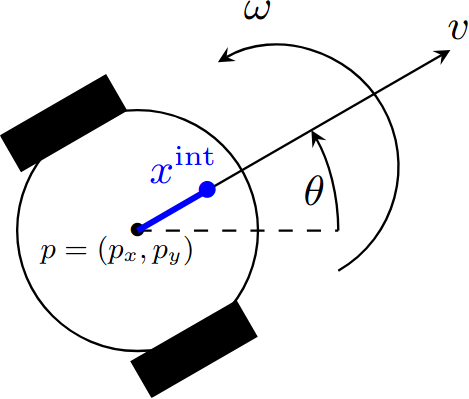
\includegraphics[width=0.2\linewidth]{./img/single_unicycle_map.png}
        \end{figure}

        By using the unicycle model dynamics, it becomes:
        \[
            \begin{split}
                \dot{\x}^\text{int} &= \begin{bmatrix}
                    \cos(\theta) & -\rho\sin(\theta) \\
                    \sin(\theta) & \rho\cos(\theta) \\
                \end{bmatrix}
                \begin{bmatrix}
                    v \\ \omega
                \end{bmatrix} \\
                \dot{\theta} &= \omega
            \end{split}
        \]

        By formulating $v$ and $\omega$ as a state-feedback control with input $\u^\text{int} \in \mathbb{R}^2$ as:
        \[
            \begin{bmatrix}
                v \\ \omega
            \end{bmatrix}
            =
            \begin{bmatrix}
                \cos(\theta) & \sin(\theta) \\
                -\frac{1}{\rho} \sin(\theta) & \frac{1}{\rho} \cos(\theta)
            \end{bmatrix} \u^\text{int}
        \]
        The result is a single-integrator $\dot{\x}^\text{int} = g(\x)\u^\text{int}$.

        A choice of $\u$ can be:
        \[
            \u^\text{int} = k (\x^\text{int} - \x^\text{dest}) + \dot{\x}^\text{dest}
        \]
\end{description}